\definecolor{pj}{HTML}{66A3FE}
\definecolor{amm}{HTML}{FFF28A}
\definecolor{an}{HTML}{52D3FA}
\definecolor{ver}{HTML}{6665FE}
\definecolor{pg}{HTML}{FF6766}
\definecolor{resp}{HTML}{FFB166}
\definecolor{pj}{HTML}{7FA8FF}

\section{Pianificazione}
\subsection{Modello adottato}
Dopo un'attenta valutazione e analisi delle esigenze del progetto, il team ha deciso di adottare un approccio di sviluppo iterativo e incrementale per la realizzazione del software richiesto. È stato quindi deciso di adoperare il modello \textit{Agile}, con particolare attenzione al framework \textit{Scrum}.\\
Avendo necessità di risposta efficace alle sfide e alle plurime esigenze dello sviluppo software, pensiamo che questo approccio sia il migliore.\\
Attraverso l'adozione dello Scrum, il team mira ad influenzare nel modo più significativo e positivo possibile il successo del progetto.

\subsection{Vantaggi adozione dello Scrum}
\begin{itemize}
    \item \textbf{Flessibilità e adattabilità}: il framework Scrum consente una rapida risposta ai cambiamenti nei requisiti del cliente, garantendo una maggiore flessibilità durante tutto il periodo di sviluppo;
    \item \textbf{collaborazione e comunicazione}: la struttura del framework incentiva una comunicazione aperta e continua tra i membri del team e le parti interessate, migliorando la comprensione reciproca, la condivisione di conoscenze e facilitando l'avanzamento dello sviluppo;
    \begin{itemize}
        \item In particolare con l’azienda proponente sono fissati \textit{SAL} (\textbf{S}tato \textbf{A}vanzamento \textbf{L}avori) ogni due settimane.       
    \end{itemize}
    \item \textbf{consegna incrementale}: attraverso la pratica di rilasci incrementali, vi è la possibilità di una distribuzione graduale delle funzionalità. Questo permette al cliente di valutare il prodotto in anticipo e di fornire feedback tempestivi;
    \item \textbf{miglioramento continuo}: il framework Scrum promuove un approccio iterativo e incrementale allo sviluppo, consentendo al team di apprendere dagli errori e di apportare miglioramenti costanti al processo di sviluppo.
\end{itemize}
La scelta di adottare il framework Scrum riflette la nostra propensione a produrre e fornire un prodotto di qualità, in modo da garantire una risposta efficiente ed efficace alle possibili nuove richieste che il cliente potrebbe avanzare.

\subsection{Gestione e monitoraggio del progetto}
In accordo con l'azienda proponente, è stato deciso di organizzare l’avanzamento del progetto in periodi di durata prefissata seguendo un approccio simile agli sprint relativi al framework Scrum.
Durante ciascun periodo di sviluppo, verranno decisi gli obiettivi da raggiungere e le attività da svolgere, in accordo con l'azienda proponente e i membri del team. La scelta degli obiettivi e attività da portare a termine durante il periodo saranno scelte attraverso un'accurata analisi che comprenderà:
\begin{itemize}
    \item l'\textbf{importanza strategica} delle attività;
    \item la \textbf{fattibilità di completare le attività} entro la durata del periodo di riferimento.
\end{itemize}
Nel remoto caso in cui alcune attività non debbano essere portate a termine nei termini indicati, queste verranno riportate nel consuntivo di periodo e proseguiranno nel periodo successivo. Ogni periodo sarà documentato attraverso una tabella esaustiva in cui saranno identificate le task relative a ciascun ruolo. Per ogni attività verrà indicato lo stato di completamento, i tempi previsti ed effettivi, e i costi associati. Al termine di ciascun periodo, sarà calcolato il costo totale del progetto fino a quel momento, fornendo una chiara visione del progresso complessivo.
Inoltre ogni periodo conterrà una discussione sui rischi occorsi e sull’esito della loro mitigazione seguendo quanto definito nella sezione apposita.
I dati riportati per ciascun periodo rappresentano un riepilogo delle informazioni inserite durante la fase di pianificazione e di preventivazione da parte del responsabile, nonché delle registrazioni orarie effettuate autonomamente dai membri del team tramite un'apposita funzione di \href{https://7last.github.io/docs/rtb/documentazione-interna/glossario#clickup}{ClickUp\textsubscript{G}}.

\subsection{Periodi}
Per ogni periodo si riportano di seguito le seguenti informazioni:
\begin{itemize}
    \item data di inizio, data di fine prevista, data di fine attuale ed eventuali giorni di ritardo;
    \item pianificazione delle attività da svolgere al suo interno (avanzamento atteso), con tanto di potenziali rischi;
    \item tempo stimato per poter completare tutte le attività previste;
    \item confronto fra il lavoro svolto (avanzamento conseguito) e quello preventivato, con annessa analisi dei costi;
    \item rischi effettivamente occorsi, valutandone il loro impatto e la loro mitigazione;
    \item retrospettiva di periodo per capire cosa e come migliorare in futuro e cosa invece mantenere;
\end{itemize}
I periodi vengono suddivisi in 3 grandi insiemi corrispondenti alle revisioni di avanzamento del progetto:
\begin{itemize}
    \item \textbf{RTB}: \textit{\textbf{R}equirements and \textbf{T}echnology \textbf{B}aseline};
    \item \textbf{PB}:  \textit{\textbf{P}roduct \textbf{B}aseline};
    \item \textbf{CA}:  \textit{\textbf{C}ustomer \textbf{A}cceptance}.
\end{itemize}

\subsection{Requirements and Technology Baseline}
\subsubsection{Primo sprint:}
\begin{itemize}
    \item Inizio: 2024-04-03;
    \item Fine: 2024-04-19;
    \item Fine attuale: 2024-04-16;
    \item Giorni di ritardo: Nessuno.
\end{itemize}
\subsubsubsection{Pianificazione} 
Durante questo periodo, il team si concentra sul dedicare risorse significative allo sviluppo, alla standardizzazione e all'automazione dei processi, ove possibile. Nel primo incontro con l'azienda proponente vengono definiti gli obiettivi chiave da raggiungere entro il prossimo SAL del 19 aprile 2024. \\In particolare, questi obiettivi comprendono:
\begin{itemize}
    \item simulazione di un sensore mediante codice \textbf{Python};
    \item integrazione con \textbf{Apache Kafka} utilizzando ambiente \textbf{Docker}.
\end{itemize}
Parallelamente a questa fase, l'amministratore ha stanziato risorse per automatizzare il processo di compilazione dei sorgenti LateX una volta caricati sul repository condiviso, e per distinguere automaticamente le parole presenti nel \href{https://7last.github.io/docs/rtb/documentazione-interna/glossario#glossario}{glossario\textsubscript{G}} da quelle che non lo sono.

\subsubsubsubsection{Rischi attesi}
I rischi attesi per questo periodo sono:
\begin{itemize}
    \item Imprecisione nella pianificazione delle attività (Rischio RO1);
    \item Elevati costi delle attività (Rischio RO3);
    \item Rischio di conflitti interni (Rischio RC1);
    \item Problemi di comunicazione (Rischio RC2);
    \item Inesperienza nell'uso delle tecnologie adottate (Rischio RT1).
\end{itemize}
Ciò è causato dal fatto che, poiché siamo ancora all'inizio del progetto, non abbiamo ancora una chiara idea di come organizzarci per ottimizzare l'uso del tempo e delle risorse.
\newpage
\subsubsubsection{Preventivo}
Ruoli coinvolti: Amministratore (Am), Responsabile (Re), Verificatore (Ve), Analista (An), Programmatore (Pg)
\begin{table}[!h]
    \centering
    \begin{tabular}{ | l | c | c | c | c | c | c | c | } 
        \hline
        \textbf{} & \textbf{Am} & \textbf{Re} & \textbf{Ve} &\textbf{An} & \textbf{Pg} & \textbf{Pj} & \textbf{Totale per persona} \\
        \hline 
        Baldo            &  -   &  -   &  -   &  -   &  7   &  -   &  7   \\ 
        Benetazzo        &  7.5 &  -   &  -   &  -   &  -   &  -   &  7.5 \\ 
        Ferro            &  -   &  -   &  -   &  -   & 10   &  -   & 10   \\ 
        Malgarise        &  -   &  -   &  -   &  7   &  -   &  -   &  7   \\ 
        Occhinegro       &  -   &  -   &  9   &  -   &  -   &  -   &  9   \\ 
        Seganfreddo      &  -   &  -   &  -   &  7   &  -   &  -   &  7   \\
        Tiozzo           &  -   &  7.5 &  -   &  -   &  -   &  -   &  7.5 \\ 
        \hline
        Totale per ruolo &  7.5 &  7.5 &  9   & 14   & 17   &  -   &  -   \\
        \hline
    \end{tabular}
    \caption{Preventivo orario per ruolo di ciascun membro del team durante il primo sprint}
    \label{tab:1}
\end{table}

%---------1_ISTOGRAMMA-----------%
\begin{figure*}
    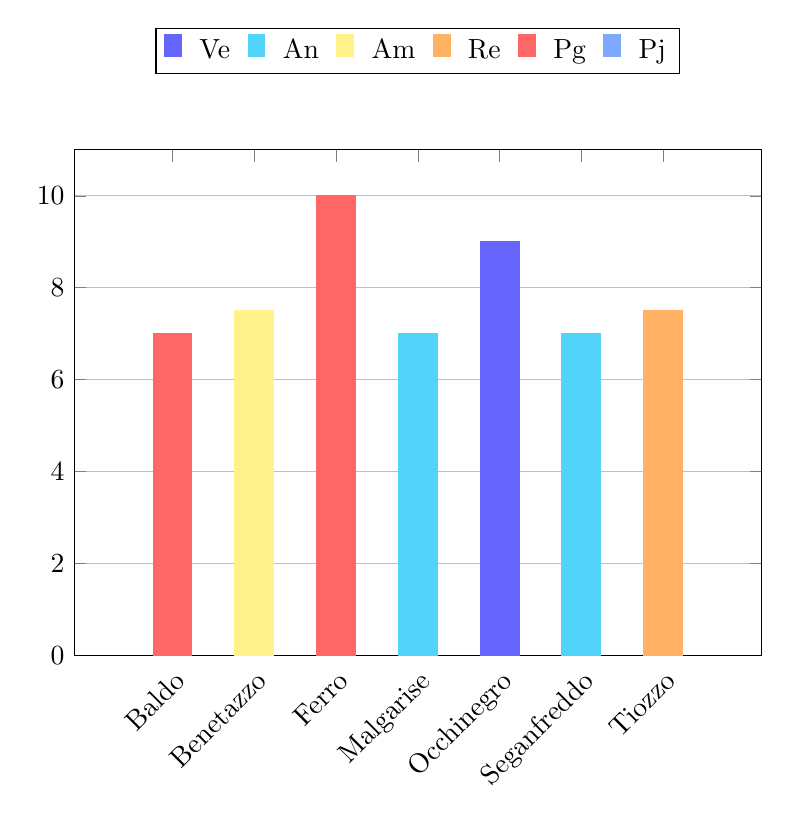
\begin{tikzpicture}
        \begin{axis}[
            width  = 0.85*\textwidth,
            height = 8cm,
            ybar stacked,
            bar width=14pt,
            ymajorgrids = true,
            symbolic x coords={Baldo, Benetazzo, Ferro, Malgarise, Occhinegro, Seganfreddo, Tiozzo},
            xtick = data,
            scaled y ticks = false,
            enlarge x limits=0.2,
            ymin=0,
            legend cell align=left,
            legend style={
                at={(0.5,1.15)},
                anchor=south,
                column sep=1ex,
                legend columns=-1
            },
            xticklabel style={rotate=45, anchor=north east, yshift=0ex, xshift=0ex},
            ]

            \addplot+[ybar, ver, fill=ver, mark=none] plot coordinates {
                (Baldo, 0)
                (Benetazzo, 0)
                (Ferro, 0)
                (Malgarise, 0)
                (Occhinegro, 9)
                (Seganfreddo, 0)
                (Tiozzo, 0)
            };
            \addplot+[ybar, an, fill=an, mark=none] plot coordinates {
                (Baldo, 0)
                (Benetazzo, 0)
                (Ferro, 0)
                (Malgarise, 7)
                (Occhinegro, 0)
                (Seganfreddo, 7)
                (Tiozzo, 0)
            };
            \addplot+[ybar, amm, fill=amm, mark=none] plot coordinates {
                (Baldo, 0)
                (Benetazzo, 7.5)
                (Ferro, 0)
                (Malgarise, 0)
                (Occhinegro, 0)
                (Seganfreddo, 0)
                (Tiozzo, 0)
            };
            \addplot+[ybar, resp, fill=resp, mark=none] plot coordinates {
                (Baldo, 0)
                (Benetazzo, 0)
                (Ferro, 0)
                (Malgarise, 0)
                (Occhinegro, 0)
                (Seganfreddo, 0)
                (Tiozzo, 7.5)
            };
            \addplot+[ybar, pg, fill=pg, mark=none] plot coordinates {
                (Baldo, 7)
                (Benetazzo, 0)
                (Ferro, 10)
                (Malgarise, 0)
                (Occhinegro, 0)
                (Seganfreddo, 0)
                (Tiozzo, 0)
            };
            \addplot+[ybar, pj, fill=pj, mark=none] plot coordinates {
                (Baldo, 0)
                (Benetazzo, 0)
                (Ferro, 0)
                (Malgarise, 0)
                (Occhinegro, 0)
                (Seganfreddo, 0)
                (Tiozzo, 0)
            };
        \legend{Ve, An, Am, Re, Pg, Pj}
        \end{axis}
    \end{tikzpicture}
    \caption{Impegno preventivo per ruolo di ciascun membro del team durante il primo periodo}
    \label{fig:1}
\end{figure*}

\newblock
%---------1_GRAFICO A TORTA-----------%
\begin{figure*}
    \centering
    \begin{tikzpicture}
        \def\printonlypositive#1{\ifdim#1pt>0pt
        #1
        \fi}
        \pie[pos={8,0},radius=3.5,sum=auto,text=legend,
        before number=\printonlypositive] {
            19.1/Verificatore,
            21.3/Analista,
            13.8/Amministratore,
            13.8/Responsabile,
            31.9/Programmatore,
             0  /Progettista
        }
        \end{tikzpicture}
    \caption{Ripartizione in percentuale dei ruoli nel primo periodo}
    \label{fig:2}
\end{figure*}

\newblock
\newpage
\subsubsubsection{Consuntivo}
Le attività previste sono state tutte svolte con successo. Abbiamo completato tutte le richieste della proponente con anticipo rispetto alla data di fine prevista.
\subsubsubsubsection{Prospetto orario}
\begin{table}[!h]
    \centering
    \begin{tabular}{ | l | c | c | c | c | c | c | c | } 
        \hline
        \textbf{} & \textbf{Am} & \textbf{Re} & \textbf{Ve} &\textbf{An} & \textbf{Pg} & \textbf{Pj} & \textbf{Totale per persona} \\
        \hline 
        Baldo            &  -   &  -   &  -   &  -   &  6   &  -   &  6   \\ 
        Benetazzo        &  6.5 &  -   &  -   &  -   &  -   &  -   &  6.5 \\ 
        Ferro            &  -   &  -   &  -   &  -   &  9   &  -   &  9   \\ 
        Malgarise        &  -   &  -   &  -   &  5   &  -   &  -   &  5   \\ 
        Occhinegro       &  -   &  -   &  9   &  -   &  -   &  -   &  9   \\ 
        Seganfreddo      &  -   &  -   &  -   &  5   &  -   &  -   &  5   \\
        Tiozzo           &  -   &  6.5 &  -   &  -   &  -   &  -   &  6.5 \\ 
        \hline
        Totale per ruolo &  6.5 &  6.5 &  9   & 10   & 15   &  -   &  -   \\
        \hline
    \end{tabular}
    \caption{Prospetto orario per ruolo di ciascun membro del team durante il primo sprint}
    \label{tab:2}
\end{table}

\newpage
\subsubsubsubsection{Prospetto economico}
\begin{table}[!h]
    \centering
    \begin{tabular}{|l| c| c| c| c| c| } 
        \hline
        \textbf{Ruolo} & \textbf{Ore} & \textbf{Costo} & \textbf{Ore rimanenti preventivo} & \textbf{Ore rimanenti consuntivo} \\
        \hline  
        Responsabile               &  6.5 &  195,00 € &  48.5 &  49.5 \\ 
        Amministratore             &  6.5 &  130,00 € &  48.5 &  49.5 \\ 
        Verificatore               &  9   &  135,00 € & 166   & 166   \\ 
        Analista                   & 10   &  250,00 € &  63   &  67   \\ 
        Programmatore              & 15   &  225,00 € & 151   & 153   \\ 
        \hline
        \textbf{Totale preventivo} & 55   & 1115,00 € & 589   &   -   \\
        \hline
        \textbf{Totale consuntivo} & 47   &  935,00 € &   -   & 597   \\
        \hline
    \end{tabular}
    \caption{Aggiornamenti economici del progetto al termine del primo periodo, riflettendo le variazioni tra preventivo e ore effettivamente lavorate}
    \label{tab:3}
\end{table}

\subsubsubsubsection{Rischi effettivamente occorsi e loro mitigazione}
\begin{table}[!h]
    \centering
    \begin{tabular}{|p{5cm}| p{2.5cm}| p{2.5cm}| p{6cm}|} 
        \hline
        \textbf{Tipologia} & \textbf{Rischio preventivato} & \textbf{Rischio non preventivato} & \textbf{Mitigazione}  \\
        \hline  
        Inesperienza del team (Rischio \textbf{RT2}) & SI & NO & Confronto con gli altri gruppi per la gestione dell'organizzazione.\\
        \hline % ???
        Impegni personali o universitari (Rischio \textbf{RO2})& NO & SI & Comunicato in anticipo gli impegni, lavoro affidato svolto o dopo l'impegno.\\
        \hline
        Inesperienza nell'uso delle tecnologie adottate (Rischio \textbf{RT3}) & SI & NO & Autoformazione e discussione interna e con la proponente.\\
        \hline
    \end{tabular}
    \caption{Rischi effettivamente occorsi e loro mitigazione durante il primo periodo}
    \label{tab:4}
\end{table}
\subsubsubsection{Retrospettiva}
La suddivisione iniziale dei ruoli per il presente sprint si è rivelata efficace e ben pensata. Ciascun componente ha lavorato senza essere sovraccaricato e il lavoro è stato distribuito in modo equo e senza disparità.\\
Durante l’ultimo sprint, un rischio inaspettato ha evidenziato la necessità di una pianificazione più accurata dei rischi nel prossimo sprint. Questo permetterà al team di evitare inconvenienti e di risparmiare tempo e risorse, che il responsabile potrà destinare ad altre attività. Ciò porterà ad un aumento dell’efficacia e dell’efficienza, riducendo i costi e i tempi di sviluppo del progetto.\\
Un'ulteriore problematica riscontrata è stata la difficoltà nell'adozione di alcune tecnologie, causando il rallentamento del lavoro. Per il prossimo sprint, si cercherà di risolvere questo problema con una maggiore formazione e con una maggiore collaborazione tra i membri del gruppo.\\
\subsubsection{Secondo sprint:}
\begin{itemize}
    \item Inizio: 2024-04-19
    \item Fine: 2024-05-06
    \item Fine attuale:
    \item Giorni di ritardo:
\end{itemize}
\subsubsubsection{Pianificazione} 
Durante il secondo periodo, il nostro team si propone di integrare "{Grafana\textsubscript{G}}" che rappresenta l'ultimo elemento dello 
{stack tecnologico\textsubscript{G}} del Proof of Concept ({POC\textsubscript{G}}), come concordato nel corso del primo {SAL\textsubscript{G}}.
Inoltre, si prevede l'implementazione della funzionalità di visualizzazione tramite grafici delle misurazioni raccolte,
assieme ad una maggiore persistenza per quanto riguarda i dati raccolti all'interno di "{ClickHouse\textsubscript{G}}".
Dal punto di vista della documentazione, invece, ci si pone l'obiettivo di portare a compimento il documento \textit{Norme di Progetto},
in modo da avere un quadro chiaro e definito delle regole e delle convenzioni da seguire durante lo sviluppo del progetto.
In concomitanza con questa attività, si prosegue con la stesura del \textit{Piano di Progetto}, in particolare con la documentazione del primo
e del secondo sprint, con l'aggiornamento continuo dei documenti \textit{Glossario} e \textit{Piano di Qualifica} e, infine,
si può procedere con la stesura del documento \textit{Analisi dei Requisiti}, con lo scopo di identificare i casi d'uso fondamentali.
Per quanto riguarda gli strumenti adottati, il team prevede di assegnare risorse per l'analisi attenta della tecnologia proposta \textit{Redpanda}
che andrebbe a sostituire \textit{Apache Kafka}, consigliata dalla proponente. Questa fase di valutazione mira a selezionare con attenzione
le tecnologie più adatte al compimento delle specifiche del capitolato.

\subsubsubsubsection{Rischi attesi}
I rischi attesi per questo periodo sono:
\begin{itemize}
    \item Inesperienza nella pianificazione delle attività (Rischio RO1);
    \item Impegni personali o universitari (Rischio RO2);
    \item Inesperienza nell'uso delle tecnologie adottate (Rischio RT1);
    \item Problemi di compatibilità tra le tecnologie adottate (Rischio RT3);
    \item Rischio di conflitti interni (Rischio RC1).
\end{itemize}
Le differenze rispetto ai rischi attesi nel primo sprint non sono così significative, questo perchè l'esperienza del gruppo è ancora acerba e limitata.
A queste si aggiungono problematiche riguardo agli impegni personali, anche legati alle festività di questo periodo. Infine l'introduzione di \textit{Grafana},
tecnologia nuova all'interno del team, potrebbe causare problemi di ineseperienza e compatibilità con le tecnologie già adottate.
\newpage
\subsubsubsection{Preventivo}
Ruoli coinvolti: Amministratore (Am), Responsabile (Re), Verificatore (Ve), Analista (An),
Programmatore (Pg), Progettista (Pj).
\begin{table}[!h]
    \centering
    \begin{tabular}{ | l | c | c | c | c | c | c | c |} 
        \hline
        \textbf{} & \textbf{Am} & \textbf{Re} & \textbf{Ve} &\textbf{An} & \textbf{Pg} & \textbf{Pj} & \textbf{Totale per persona} \\
        \hline 
        Baldo            &  5   &  -   &  -   &  -   &  -   &  -   &  5   \\ 
        Benetazzo        &  -   &  -   &  7   &  -   &  -   &  -   &  7   \\ 
        Ferro            &  -   &  -   &  -   & 10   &  -   &  -   & 10   \\ 
        Malgarise        &  -   &  6   &  -   &  -   &  -   &  -   &  6   \\ 
        Occhinegro       &  -   &  -   &  -   &  -   & 10   &  -   & 10   \\ 
        Seganfreddo      &  -   &  -   &  -   &  -   &  -   &  7   &  7   \\
        Tiozzo           &  -   &  -   &  -   &  -   & 10   &  -   & 10   \\ 
        \hline
        Totale per ruolo &  5   &  6   &  7   & 10   & 20   &  7   &  -   \\
        \hline
    \end{tabular}
    \caption{Preventivo orario per ruolo di ciascun membro del team durante il secondo sprint}
    \label{tab:5}
\end{table}

%---------1_ISTOGRAMMA-----------%
\begin{figure*}
    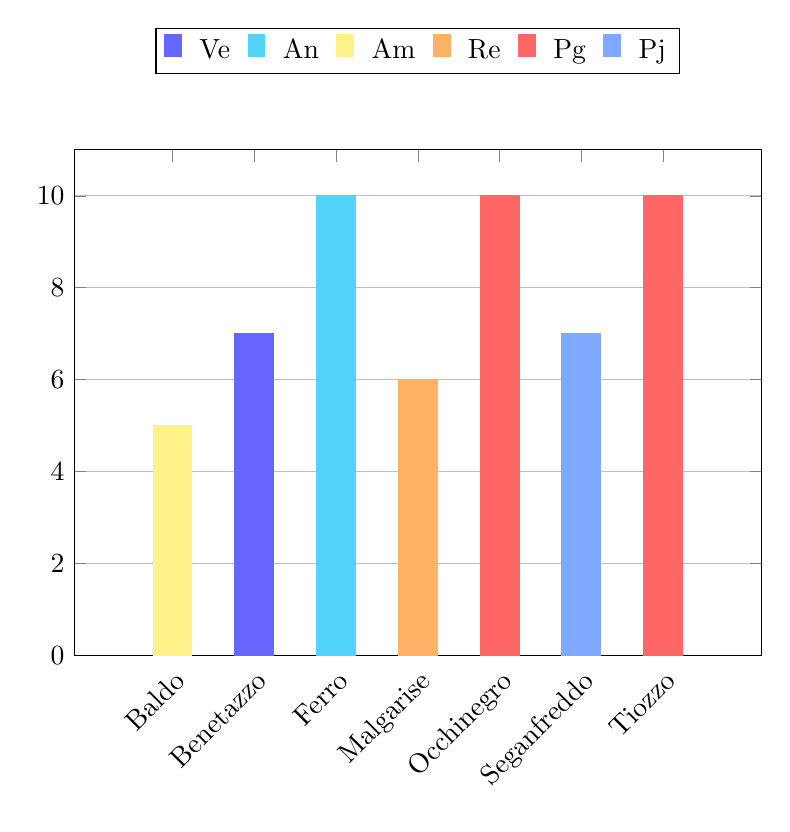
\begin{tikzpicture}
        \begin{axis}[
            width  = 0.85*\textwidth,
            height = 8cm,
            ybar stacked,
            bar width=14pt,
            ymajorgrids = true,
            symbolic x coords={Baldo, Benetazzo, Ferro, Malgarise, Occhinegro, Seganfreddo, Tiozzo},
            xtick = data,
            scaled y ticks = false,
            enlarge x limits=0.2,
            ymin=0,
            legend cell align=left,
            legend style={
                at={(0.5,1.15)},
                anchor=south,
                column sep=1ex,
                legend columns=-1
            },
            xticklabel style={rotate=45, anchor=north east, yshift=0ex, xshift=0ex},
            ]
    
            \addplot+[ybar, ver, fill=ver, mark=none] plot coordinates {
                (Baldo, 0)
                (Benetazzo, 7)
                (Ferro, 0)
                (Malgarise, 0)
                (Occhinegro, 0)
                (Seganfreddo, 0)
                (Tiozzo, 0)
            };
            \addplot+[ybar, an, fill=an, mark=none] plot coordinates {
                (Baldo, 0)
                (Benetazzo, 0)
                (Ferro, 10)
                (Malgarise, 0)
                (Occhinegro, 0)
                (Seganfreddo, 0)
                (Tiozzo, 0)
            };
            \addplot+[ybar, amm, fill=amm, mark=none] plot coordinates {
                (Baldo, 5)
                (Benetazzo, 0)
                (Ferro, 0)
                (Malgarise, 0)
                (Occhinegro, 0)
                (Seganfreddo, 0)
                (Tiozzo, 0)
            };
            \addplot+[ybar, resp, fill=resp, mark=none] plot coordinates {
                (Baldo, 0)
                (Benetazzo, 0)
                (Ferro, 0)
                (Malgarise, 6)
                (Occhinegro, 0)
                (Seganfreddo, 0)
                (Tiozzo, 0)
            };
            \addplot+[ybar, pg, fill=pg, mark=none] plot coordinates {
                (Baldo, 0)
                (Benetazzo, 0)
                (Ferro, 0)
                (Malgarise, 0)
                (Occhinegro, 10)
                (Seganfreddo, 0)
                (Tiozzo, 10)
            };
            \addplot+[ybar, pj, fill=pj, mark=none] plot coordinates {
                (Baldo, 0)
                (Benetazzo, 0)
                (Ferro, 0)
                (Malgarise, 0)
                (Occhinegro, 0)
                (Seganfreddo, 7)
                (Tiozzo, 0)
            };
            \legend{Ve, An, Am, Re, Pg, Pj}
        \end{axis}
    \end{tikzpicture}
    \caption{Impegno preventivo per ruolo di ciascun membro del team durante il secondo periodo}
    \label{fig:3}
\end{figure*}

%---------1_GRAFICO A TORTA-----------%
\begin{figure*}
    \centering
    \begin{tikzpicture}
        \def\printonlypositive#1{\ifdim#1pt>0pt
        #1
        \fi}
        \pie[pos={8,0},radius=3.5,sum=auto,text=legend,
        before number=\printonlypositive] {
            12.7/Verificatore,
            18.2/Analista,
             9.1/Amministratore,
            10.9/Responsabile,
            36.4/Programmatore,
            12.7/Progettista
        }
        \end{tikzpicture}
    \caption{Ripartizione in percentuale dei ruoli nel secondo periodo}
    \label{fig:4}
\end{figure*}

\newblock
\newpage
\subsubsubsection{Consuntivo}
Tutte le attività previste sono state svolte con successo. \textbf{[TO DO]}
Come si può notare dal prospetto orario, i Programmatori hanno richiesto più ore rispetto a quanto preventivato, al contrario, l'Analista
ha richiesto meno ore.
\subsubsubsubsection{Prospetto orario}
\begin{table}[!h]
    \centering
    \begin{tabular}{ | l | c | c | c | c | c | c | c |} 
        \hline
        \textbf{} & \textbf{Am} & \textbf{Re} & \textbf{Ve} &\textbf{An} & \textbf{Pg} & \textbf{Pj} & \textbf{Totale per persona} \\
        \hline 
        Baldo            &  5   &  -   &  -   &  -   &  -   &  -   &  5   \\ 
        Benetazzo        &  -   &  -   &  6   &  -   &  -   &  -   &  6   \\ 
        Ferro            &  -   &  -   &  -   & 10   &  -   &  -   & 10   \\ 
        Malgarise        &  -   &  6   &  -   &  -   &  -   &  -   &  6   \\ 
        Occhinegro       &  -   &  -   &  -   &  -   &  9   &  -   &  9   \\ 
        Seganfreddo      &  -   &  -   &  -   &  -   &  -   &  7   &  7   \\
        Tiozzo           &  -   &  -   &  -   &  -   &  9   &  -   &  9   \\ 
        \hline
        Totale per ruolo &  5   &  6   &  6   & 10   & 18   &  7   &  -   \\
        \hline
    \end{tabular}
    \caption{Prospetto orario per ruolo di ciascun membro del team durante il secondo sprint}
    \label{tab:6}
\end{table}

\newpage
\subsubsubsubsection{Prospetto economico} %verificare correttezza dati inseriti
\begin{table}[!h]
    \centering
    \begin{tabular}{|l| c| c| c| c| c| } 
        \hline
        \textbf{Ruolo} & \textbf{Ore} & \textbf{Costo} & \textbf{Ore rimanenti preventivo} & \textbf{Ore rimanenti consuntivo} \\
        \hline  
        Responsabile               &  6   &  180,00 € &  41.5 &  42.5 \\ 
        Amministratore             &  5   &  100,00 € &  42.5 &  43.5 \\ 
        Verificatore               &  6   &   90,00 € & 158   & 158   \\ 
        Analista                   & 10   &  250,00 € &  56   &  59   \\ 
        Programmatore              & 18   &  270,00 € & 133   & 134   \\
        Progettista                &  7   &  175,00 € & 105   & 105   \\
        \hline
        \textbf{Totale preventivo} & 55   & 1110,00 € & 534   &   -   \\
        \hline
        \textbf{Totale consuntivo} & 55   & 1065,00 € &   -   & 545   \\
        \hline
    \end{tabular}
    \caption{Aggiornamenti economici del progetto al termine del secondo periodo, riflettendo le variazioni tra preventivo e ore effettivamente lavorate}
    \label{tab:7}
\end{table}

\subsubsubsubsection{Rischi effettivamente occorsi e loro mitigazione}
\subsubsubsection{Retrospettiva}
\subsubsection{Terzo sprint:}
\begin{itemize}
    \item Inizio: 2024-04-25
    \item Fine: 2024-05-09
    \item Fine attuale:
    \item Giorni di ritardo:
\end{itemize}

\subsubsubsection{Pianificazione} 
SCRIVI QUALCOSA A RIGUARDO (PT. 4.1.1.1 DEGLI OVERTURE)

\subsubsubsubsection{Rischi attesi}
I rischi attesi per questo periodo sono:
\begin{itemize}
    \item Inesperienza del team
    \item Imprecisione nella pianificazione delle attività
    \item Elevati costi delle attività
    \item Rischio di conflitti interni 
    \item problemi di comunicazione
    \item problemi di coordinamento
\end{itemize}
Questo perchè, essendo all’inizio del progetto, siamo ancora incerti su molti aspetti di quest’ultimo, ci stiamo attualmente organizzando e dobbiamo apprendere ancora molto, dunque la probabilità di incorrere in qualche problema tra quelli riportati è abbastanza elevata.

\subsubsubsection{Preventivo}
Ruoli coinvolti:

\subsubsubsection{Consuntivo}
Le attività previste sono state tutte svolte con successo

\subsubsubsubsection{Prospetto orario}

\subsubsubsubsection{Prospetto economico}

\subsubsubsubsection{Rischi effettivamente occorsi e loro mitigazione}

\subsubsubsection{Retrospettiva}

\subsubsection{Quarto sprint:}
\begin{itemize}
    \item Inizio: 2024-05-10
    \item FIne: 2024-05-24
    \item Fine attuale:
    \item Giorni di ritardo:
\end{itemize}

\subsubsubsection{Pianificazione} 
SCRIVI QUALCOSA A RIGUARDO (PT. 4.1.1.1 DEGLI OVERTURE)

\subsubsubsubsection{Rischi attesi}
I rischi attesi per questo periodo sono:
\begin{itemize}
    \item Inesperienza del team
    \item Imprecisione nella pianificazione delle attività
    \item Elevati costi delle attività
    \item Rischio di conflitti interni 
    \item problemi di comunicazione
    \item problemi di coordinamento
\end{itemize}
Questo perchè, essendo all’inizio del progetto, siamo ancora incerti su molti aspetti di quest’ultimo, ci stiamo attualmente organizzando e dobbiamo apprendere ancora molto, dunque la probabilità di incorrere in qualche problema tra quelli riportati è abbastanza elevata.

\subsubsubsection{Preventivo}
Ruoli coinvolti:

\subsubsubsection{Consuntivo}
Le attività previste sono state tutte svolte con successo

\subsubsubsubsection{Prospetto orario}

\subsubsubsubsection{Prospetto economico}

\subsubsubsubsection{Rischi effettivamente occorsi e loro mitigazione}

\subsubsubsection{Retrospettiva}

\subsubsection{Quinto sprint:}
\begin{itemize}
    \item Inizio: 2024-05-25
    \item FIne: 2024-06-09
    \item Fine attuale:
    \item Giorni di ritardo:
\end{itemize}

\subsubsubsection{Pianificazione} 
SCRIVI QUALCOSA A RIGUARDO (PT. 4.1.1.1 DEGLI OVERTURE)

\subsubsubsubsection{Rischi attesi}
I rischi attesi per questo periodo sono:
\begin{itemize}
    \item Inesperienza del team
    \item Imprecisione nella pianificazione delle attività
    \item Elevati costi delle attività
    \item Rischio di conflitti interni 
    \item problemi di comunicazione
    \item problemi di coordinamento
\end{itemize}
Questo perchè, essendo all’inizio del progetto, siamo ancora incerti su molti aspetti di quest’ultimo, ci stiamo attualmente organizzando e dobbiamo apprendere ancora molto, dunque la probabilità di incorrere in qualche problema tra quelli riportati è abbastanza elevata.

\subsubsubsection{Preventivo}
Ruoli coinvolti:

\subsubsubsection{Consuntivo}
Le attività previste sono state tutte svolte con successo

\subsubsubsubsection{Prospetto orario}

\subsubsubsubsection{Prospetto economico}

\subsubsubsubsection{Rischi effettivamente occorsi e loro mitigazione}

\subsubsubsection{Retrospettiva}

\subsubsection{Sesto sprint:}
\begin{itemize}
    \item Inizio: 2024-06-10
    \item FIne: 2024-06-24
    \item Fine attuale:
    \item Giorni di ritardo:
\end{itemize}

\subsubsubsection{Pianificazione} 
SCRIVI QUALCOSA A RIGUARDO (PT. 4.1.1.1 DEGLI OVERTURE)

\subsubsubsubsection{Rischi attesi}
I rischi attesi per questo periodo sono:
\begin{itemize}
    \item Inesperienza del team
    \item Imprecisione nella pianificazione delle attività
    \item Elevati costi delle attività
    \item Rischio di conflitti interni 
    \item problemi di comunicazione
    \item problemi di coordinamento
\end{itemize}
Questo perchè, essendo all’inizio del progetto, siamo ancora incerti su molti aspetti di quest’ultimo, ci stiamo attualmente organizzando e dobbiamo apprendere ancora molto, dunque la probabilità di incorrere in qualche problema tra quelli riportati è abbastanza elevata.

\subsubsubsection{Preventivo}
Ruoli coinvolti:

\subsubsubsection{Consuntivo}
Le attività previste sono state tutte svolte con successo

\subsubsubsubsection{Prospetto orario}

\subsubsubsubsection{Prospetto economico}

\subsubsubsubsection{Rischi effettivamente occorsi e loro mitigazione}

\subsubsubsection{Retrospettiva}

\subsubsection{Settimo sprint:}
\begin{itemize}
    \item Inizio: 2024-06-25
    \item FIne: 2024-07-09
    \item Fine attuale:
    \item Giorni di ritardo:
\end{itemize}

\subsubsubsection{Pianificazione} 
SCRIVI QUALCOSA A RIGUARDO (PT. 4.1.1.1 DEGLI OVERTURE)

\subsubsubsubsection{Rischi attesi}
I rischi attesi per questo periodo sono:
\begin{itemize}
    \item Inesperienza del team
    \item Imprecisione nella pianificazione delle attività
    \item Elevati costi delle attività
    \item Rischio di conflitti interni 
    \item problemi di comunicazione
    \item problemi di coordinamento
\end{itemize}
Questo perchè, essendo all’inizio del progetto, siamo ancora incerti su molti aspetti di quest’ultimo, ci stiamo attualmente organizzando e dobbiamo apprendere ancora molto, dunque la probabilità di incorrere in qualche problema tra quelli riportati è abbastanza elevata.

\subsubsubsection{Preventivo}
Ruoli coinvolti:

\subsubsubsection{Consuntivo}
Le attività previste sono state tutte svolte con successo

\subsubsubsubsection{Prospetto orario}

\subsubsubsubsection{Prospetto economico}

\subsubsubsubsection{Rischi effettivamente occorsi e loro mitigazione}

\subsubsubsection{Retrospettiva}

\subsubsection{Sommario finale}

\subsubsubsection{Riepilogo prospetto orario}

\subsubsubsubsection{Ore consumate}

\subsubsubsubsection{Ore rimanenti}

\subsubsubsection{Riepilogo prospetto economico}

\subsubsubsection{Costi totali}

\subsection{Tra RTB e PB}

\subsubsection{Ottavo periodo}
\begin{itemize}
    \item Inizio: 2024-07-10
    \item FIne: 2024-07-24
    \item Fine attuale:
    \item Giorni di ritardo:
\end{itemize}

\subsubsubsection{Pianificazione} 
SCRIVI QUALCOSA A RIGUARDO (PT. 4.1.1.1 DEGLI OVERTURE)

\subsubsubsubsection{Rischi attesi}
I rischi attesi per questo periodo sono:
\begin{itemize}
    \item Inesperienza del team
    \item Imprecisione nella pianificazione delle attività
    \item Elevati costi delle attività
    \item Rischio di conflitti interni 
    \item problemi di comunicazione
    \item problemi di coordinamento
\end{itemize}
Questo perchè, essendo all’inizio del progetto, siamo ancora incerti su molti aspetti di quest’ultimo, ci stiamo attualmente organizzando e dobbiamo apprendere ancora molto, dunque la probabilità di incorrere in qualche problema tra quelli riportati è abbastanza elevata.

\subsubsubsection{Preventivo}
Ruoli coinvolti:

\subsubsubsection{Consuntivo}

\subsubsubsubsection{Prospetto orario}

\subsubsubsubsection{Prospetto economico}

\subsubsubsubsection{Rischi effettivamente occorsi e loro mitigazione}

\subsubsubsection{Retrospettiva}
